\documentclass{article}
\usepackage[utf8]{inputenc}
\usepackage{tabularx}
\usepackage{longtable}
\usepackage[margin=3cm]{geometry}
\usepackage{biblatex}
\usepackage{titling}
\usepackage{hyperref}
\usepackage{float}
\usepackage{graphicx}
\usepackage{import}
\usepackage{color}
% \usepackage{stfloats}
% \usepackage{dblfloatfix}
% \usepackage[dvisvgm, usenames, dvipsnames]{color}

\setlength{\droptitle}{-2cm}

\bibliography{source} 
% A comparative study of pose estimation techniques on point clouds from high DOF humanoid gripper tactile sensors

\title{Object Pose Estimation from High DOF Humanoid Gripper Tactile Sensors using Features Found by In-Hand Manipulation}
\author{\vspace{-1cm}}
\date{\vspace{-1cm}}

\begin{document}
\maketitle

\begin{flushleft}
\begin{tabular}{@{} p{\dimexpr 0.5\linewidth-2\tabcolsep} p{\dimexpr 0.5\linewidth-2\tabcolsep} @{}} 
 \textbf{Student}     & Victor Melbye Staven \\ \\
 \textbf{Supervisor}  & Christoffer Sloth \\ \\
 \textbf{Start Date}  & 1 September 2022 \\ \\
 \textbf{End Date}    & 3 June 2023 \\ \\
 \textbf{ECTS}        & 40 \\ \\
 \textbf{Institution} & University of Southern Denmark, The Technical Faculty (TEK)
\end{tabular}
\end{flushleft}

\newpage

\section*{Project Description}
\label{project-description}
The structure of this section is to present the context of the project followed by which problem has been identified along with the corresponding sub-problems needed to be solved. Related work will here be presented along with suggested techniques which, given the current understanding, would provide solutions to the found sub-problems. Finally an expected timeline of the project in its entirety will be presented. 

\subsection*{Context}
\label{context}
\begin{minipage}{0.5\textwidth}
Within robotics a common and well researched problem is bin picking, which often is solved using computer vision (CV) techniques to pose estimate objects. These techniques however suffer from the weaknesses of CV such as outliers in solving the correspondence problem. Here specifically occlusions, reflecting, transparent or homogeneous surfaces, and repetitive structures are common problems which as of the writing of this project have jet to be completely solved.\par
This project attempts to solve the pose estimation problem by processing tactile sensor inputs from a humanoid robot hand, more specifically a Shadow Dexterous Hand\cite{shadow-dex-hand} with 20 degrees of freedom (DOF). Using tactile inputs rather than visual, eliminates the weaknesses mentioned above. A schematic showing the hand can be seen in figure \ref{fig:shadow-dex-hand}
\end{minipage} \hfill
\begin{minipage}{0.45\textwidth}
\begin{figure}[H]
\centering
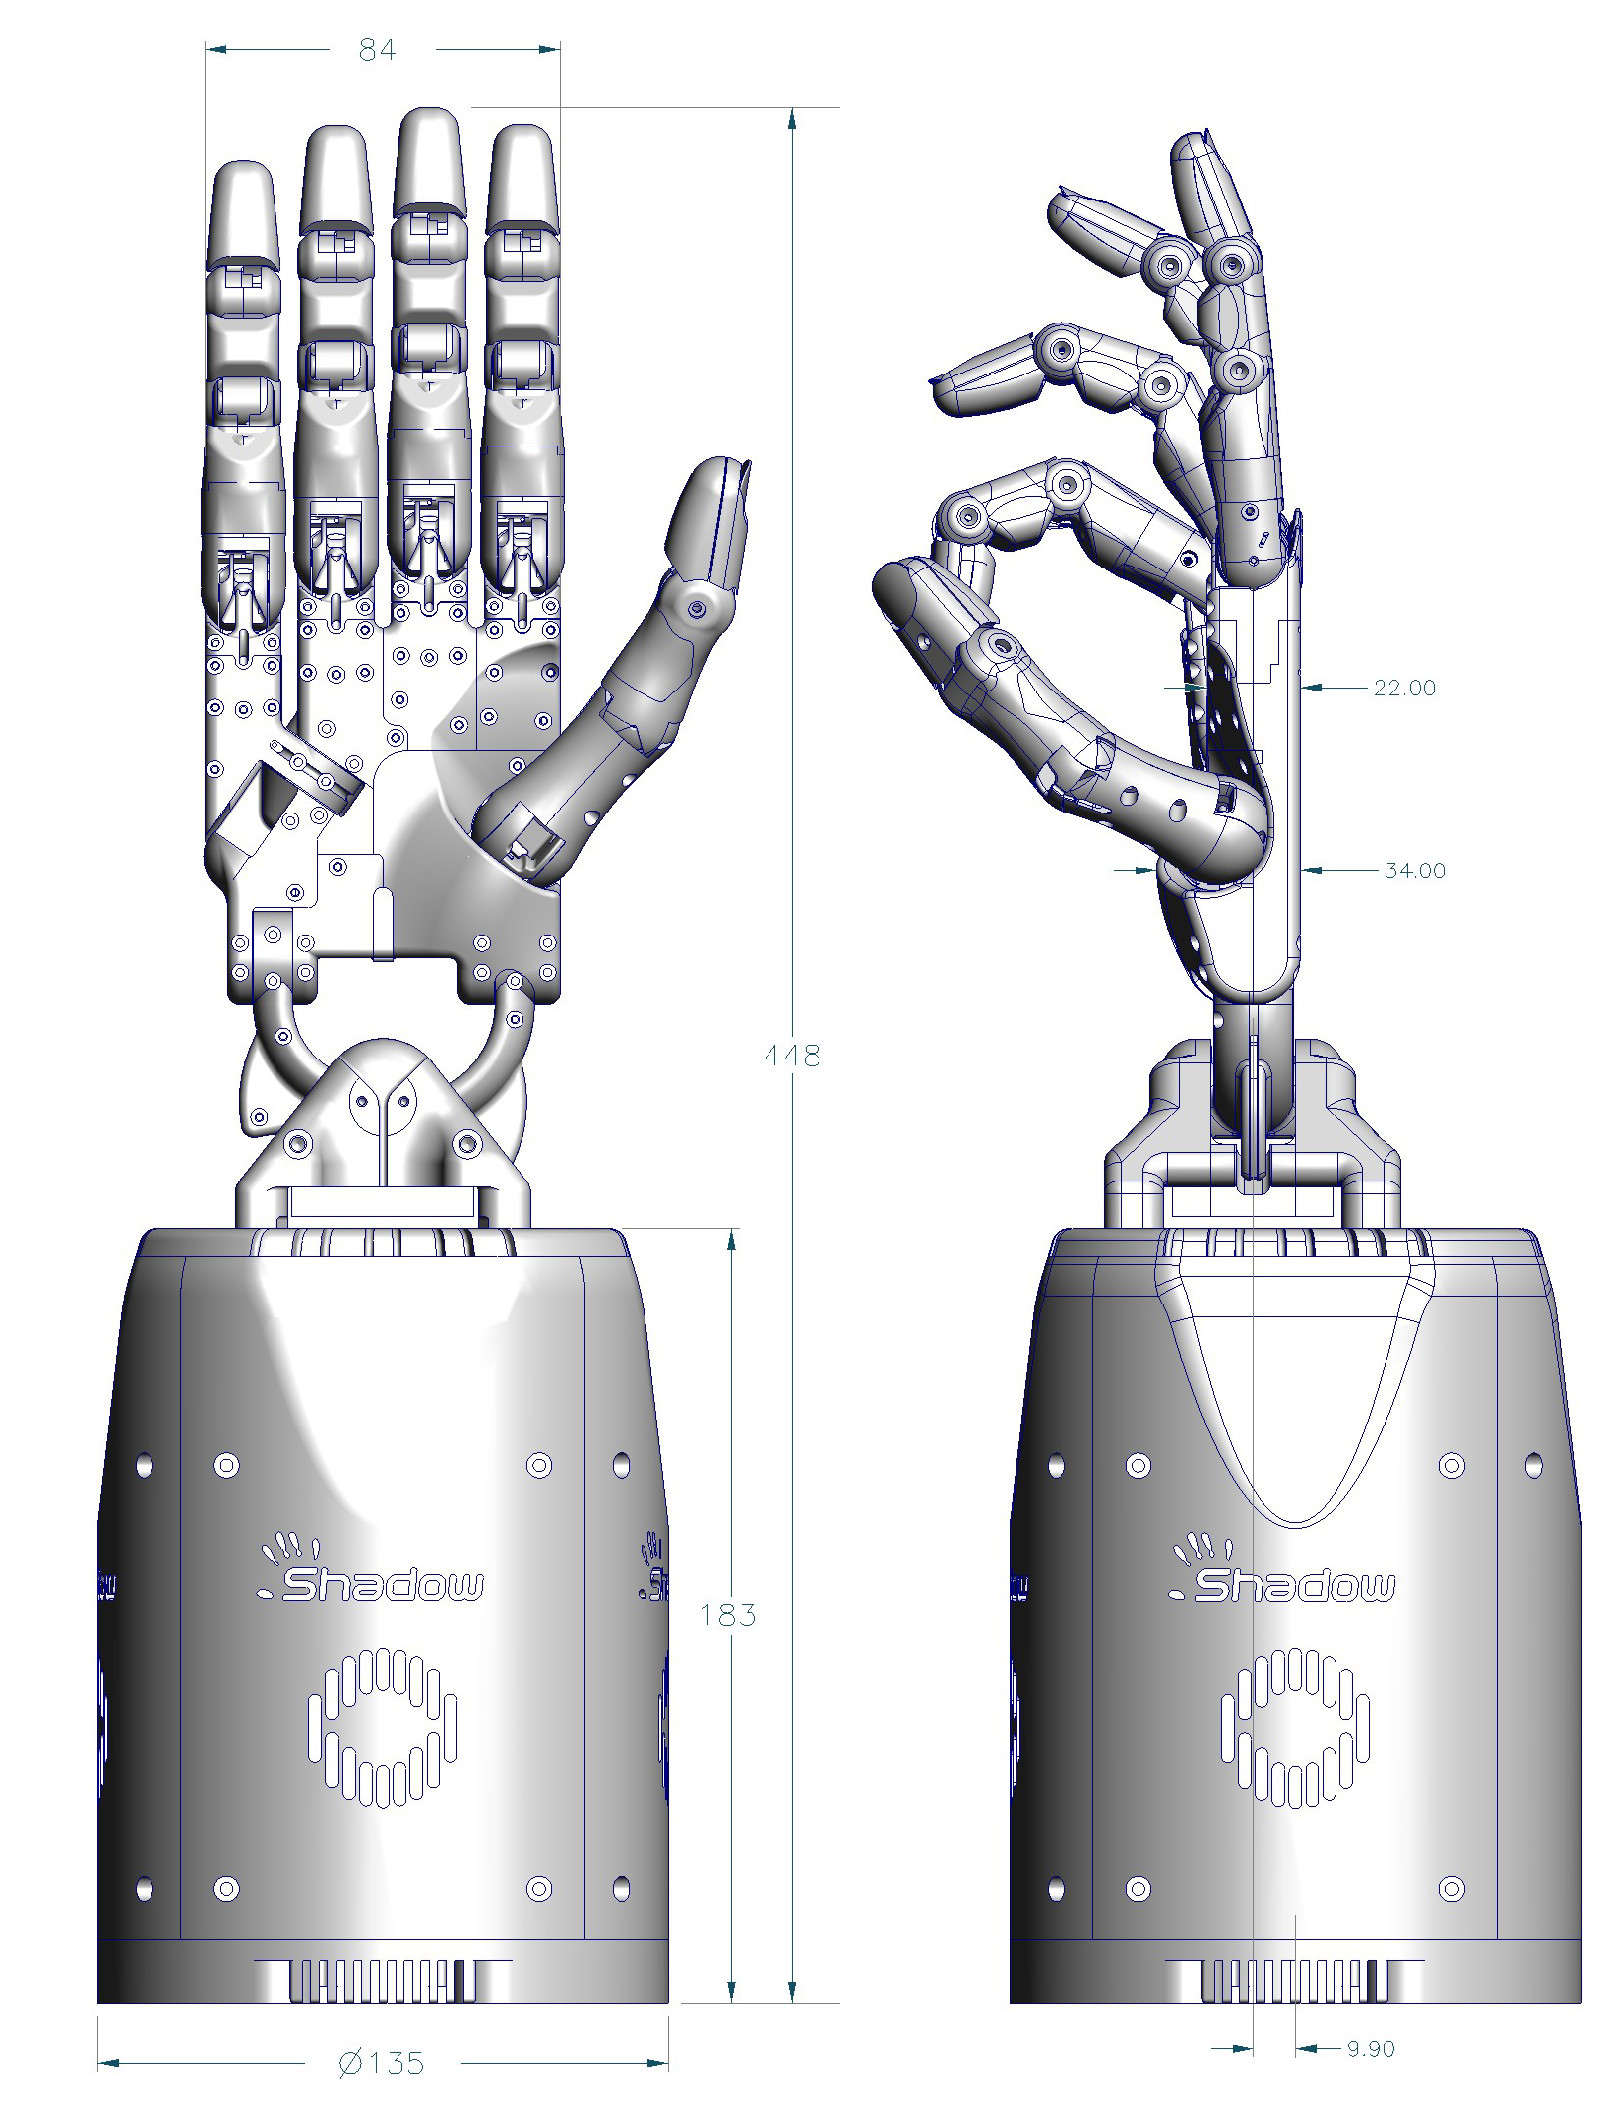
\includegraphics[height=\textwidth]{figs/shadow-dex-hand.jpg}
\caption{ Shadow dexterous hand \\ from Shadow Robots\cite{shadow-dex-hand} }
\label{fig:shadow-dex-hand}
\end{figure}
\end{minipage}

\subsection*{Problem}
\label{subsec:problem}

Using this approach, the overall problem can be partitioned into 3 sub-problems labeled problem 1, 2 and 3. \par
Problem 1 involves modeling the contact between the gripper's fingers and the object. Problem 2 is to convert the data collected through the contact model to meaningful surface data, treat these data as features and use these to estimate pose candidates. Finally problem 3 involves in-hand manipulation, such that further information is gained by probing the object. Here new desired surface points are found such that strong surface features are found to better identify the object's correct pose.

% Problem 1 involves control of the hand in such a manner that in-hand manipulation can be done to make the object stay within the gripper's grasp. Using these grasps the tactile sensors can generate enough useful contact points with the object to make up a point cloud. Each point here can also be ascribed extra features such as the force measured by the sensor when making contact with the object. \par
% Problem 2 is to align the found point cloud with the known ground truths to determine its transformation, and thus its pose within the gripper. Once the best alignment has been found, the same object label associated with the best fit is ascribed to the object in hand. 

\subsection*{Related Work}
\label{related-work}

Within the field of robotics the problem of in-hand pose estimation is separated into different categories based on the methods applied. Here the approaches which address the sub-problems presented in Problem will be considered. To solve problem 1 two different models are generally used for representing the contact information: point-cloud based\cite{tracking-objects-with-point-clouds-from-vision-and-touch} and image-based \cite{tactile-mapping-and-localization-from-high-resolution-tactile-imprints} tactile information. The point-cloud based approaches are generally preferred in hybrid systems with vision.\par
For problem 2 one method for feature mapping include global tactile and shape mapping \cite{tactile-mapping-and-localization-from-high-resolution-tactile-imprints}. This method can localize the sensor point cloud in the world’s frame by assuming that the transformation between sensor, gripper and robot arm is rigid and calibrated. The point clouds generated from the measurements are then stitched together into a single point cloud. A different approach is to use the found measurements and treat them as features for a optimization solver to align a sampled model and the measured data. One such optimization technique is GNC \cite{graduated-non-convexity-for-robust-spatial-perception}. \par
Problem 3 presents challenges of significant magnitude due to the complexity of modelling gripper and object in contact and of coordinating finger motion for complex manipulation actions. From this different approaches has emerged involving reinforcement learning \cite{learning-dexterous-in-hand-manipulation}, hierarchical control \cite{learning-hierarchical-control-for-robust-in-hand-manipulation} and control optimization \cite{planning-in-hand-object-manipulation-with-multifingered-hands-considering-task-constraints}.

%  + G LOBAL T ACTILE A ND S HAPE M APPING\cite{tactile-mapping-and-localization-from-high-resolution-tactile-imprints}
%  + gnc \cite{graduated-non-convexity-for-robust-spatial-perception}
%  + 

% we fuse the tactile imprints and
% the kinematics (gripper pose and opening) of multiple
% grasps of a fixed object to reconstruct its global tactile
% shape. This includes the object geometric shape as well
% as a discrete representation of its tactile imprints. We
% validate the algorithm in Section V by recovering the
% main dimensions of known objects with an error lower
% than 5%.

% image-based tactile sensors
% local contact shapes from
% objects to build a map of the object and then use it to localize new contacts. The approach is meant
% to deal with small parts with discriminative features.

% These include approaches using deep learning, Bayesian methods, computer vision, tactile sensing and combinations of these. Methods also exist for using contact with the environment causing a measured force in a force torque sensor\cite{contact-based-in-hand-pose-estimation-using-bayesian-state-estimation-and-particle-filtering}

%  + using texture discrimination and bayssian exploration
%   + This study is focused on texture discrimination, a subset of a much larger group of exploratory movements and percepts that humans use to discriminate, characterize, and identify objects.\cite{bayesian-exploration-for-intelligent-identification-of-textures}

%  + vision based methods DL
%   + utilize visual and contact information adaptively to maximally reduce the uncertainty about the in-hand object pose in a Bayesian state estimation framework. As most of the uncertainty can be resolved from visual observations, our approach reduces the number of physical environment interactions while keeping a high pose estimation accuracy.\cite{visuotactile-6d-pose-estimation-of-an-in-hand-object-using-vision-and-tactile-sensor-data}
%   + see 86 87 in review
  
  
%  + Pure tactile with DL
%   + method not making assumptions based on object localization. Our key insight is that an object is composed of several local surface patches, each informative enough to achieve reliable object tracking.\cite{patchGraph-in-hand-tactile-tracking-with-learned-surface-normals}


%  Local shape recognition



\subsection*{Proposed Solution}
\label{proposed-solution}

To solve the problem presented for this project the work will be done in simulation using kinematic models of the robot hand and the object of interest. Here the pose estimation will only be done on one object type for simplicity.
For problem 1 the solution chosen is the tactile image-based contact model, due to the promising results showing in similar applications as referenced in Related Work. The solution methods chosen for problem 2 is GNC due to its high robustness and low computation time is as presented. Finally optimization based control of the robot hand is chosen as the solution for problem 3. 


% To solve problem 1 the model representation chosen is the image-based tactile sensing format, as this has been used in similar applications as presented in Related Work. Problem 2 

% 1) what are we dealing with?
%     + simulation first
%     + kinematic model of object and gripper

% robot hand control
% To solve problem 1 different control approaches have been researched within the literature, some involving methods from artificial intelligence (AI) more specifically using reinforcement learning (RL) \cite{learning-dexterous-in-hand-manipulation}, others revolve around more analytical approaches, such as the use of extrinsic forces to perform in hand manipulation\cite{extrinsic-dexterous-hand} or using a sequence of predefined manipulation skills \cite{surprisingly-robust-in-hand-manipulation-an-empirical-study}. 
% Approaches which combine the classical control methods with deep RL have also been developed, such that a hierarchical structure is used as task abstraction \cite{learning-hierarchical-control-for-robust-in-hand-manipulation}.
% The method chosen for this project is classical control techniques \cite{handbook-of-robotics}.\par
% Solutions addressing problem 2 involves comparing 3 different techniques. The methods chosen for this project are: 3D histograms generation based on point triangulation \cite{a-triangle-histogram-for-object-classification-by-tactile-sensing}, tactile shape reconstruction (TSR) using a probabilistic approach\cite{a-probabilistic-approach-to-tactile-shape-reconstruction} and graduated non-convexity which utilizes robust non-minimal optimization techniques for point cloud alignment\cite{graduated-non-convexity-for-robust-spatial-perception}.

\subsection*{Timeline}
The expected timeline for the project can be seen in figure \ref{suggested-project-timeline} where the deadline for solving problem 1 is the first of January 2023 meaning an estimated 4 months is needed to solve this problem. Likewise 4 months are reserved for solving problem 2, ending with one month for finishing the report.

\begin{figure}[h!]
\centering
\import{figs/}{master-project-flow-v2.pdf_tex}
\caption{Suggested project timeline}
\label{suggested-project-timeline}
\end{figure}


\begin{center}
    \vspace{10cm}
    \begin{figure}[b!]
    \begin{tabular}{@{}p{0.5\textwidth} p{1cm} p{0.3\textwidth}@{}}
    \hrulefill & & \hrulefill \\
    Victor Melbye Staven & & Date \\ \\ \\ \\
    \hrulefill & & \hrulefill \\
    Christoffer Sloth & & Date \\
    \end{tabular}
    \end{figure}
\end{center}

\clearpage

% \begin{center}
% % \vspace{5cm}
% \begin{tabular}[b!]{@{}p{0.5\textwidth} p{1cm} p{0.3\textwidth}@{}}
% \hrulefill & & \hrulefill \\
% Victor Melbye Staven & & Date \\ \\ \\ \\
% \hrulefill & & \hrulefill \\
% Christoffer Sloth & & Date \\
% \end{tabular}
% \end{center}

\newpage
\printbibliography

\end{document}
